\documentclass{homework}
\usepackage{xcolor}
\usepackage{nicematrix}
\usepackage{booktabs}
\usepackage{enumitem}
\usepackage{caption}
\usepackage{subcaption}
\usepackage{leftidx}
\usepackage{tikz}

\NiceMatrixOptions{cell-space-limits = 1pt}

\title{Solutions Excercise 2}
\author{
  Maksimov, Dmitrii\\
  \texttt{dmitrii.maksimov@fau.de}
  \and
  Ilia, Dudnik\\
  \texttt{ilia.dudnik@fau.de}
}

\begin{document}

\maketitle

\exercise
The \emph{k-SAT} problem is defined as follows:
\begin{itemize}
\item \underline{Given:} Let $\mathcal{F}$ be a Boolean CNF formula where each clause contains exactly \emph{k} literals.
\item \underline{Question:} Is $\mathcal{F}$ satisfiable?
\end{itemize}
\begin{enumerate}[label=(\alph*)]
	\item Show: 3-SAT is $\mathcal{NP}$-complete.
	
	3-SAT is $\mathcal{NP}$-complete if it is a $\mathcal{NP}$-hard and also 3-SAT $\in \mathcal{NP}$.
	\begin{enumerate}[label = \arabic*.]
		\item Proof of 3-SAT $\in \mathcal{NP}$

		3-SAT is a subset of SAT and we know that SAT is $\mathcal{NP}$.
		\[\text{3-SAT} \subseteq \text{SAT} \in \mathcal{NP} \Rightarrow \text{3-SAT} \in \mathcal{NP}\]
		\item Proof of 3-SAT is a $\mathcal{NP}$-hard
		
		3-SAT is a $\mathcal{NP}$-hard if for every $L'\in \mathcal{NP}$, there is a Karp reduction from \emph{L'} to 3-SAT. Let us see that SAT can be reduced to 3-SAT in polynomial time: \[\text{SAT}\leq_p \text{3-SAT}.\]
		The original SAT problem is: \[\upphi = C_1\land C_2\land \dots \land C_n, \] where $\upphi$ is satisfiable if every clause $C_i$ is satisfiable and $C_i=(v_1\lor \dots \lor v_m), m = k$. Let us find an alogorithm $R$ for $k=1, k=2, k>3$.
	\begin{itemize}
		\item $k=1$

		Let $z_1$ and $z_2$ be two new variables. Replace $C_i$ by the following four clauses:
		\[C'_i = (v\lor z_1\lor z_2)\cdot(v\lor \overline{z_1}\lor z_2)\cdot(v\lor z_1\lor \overline{z_2})\cdot(v\lor \overline{z_1}\lor \overline{z_2}). \]
		The truth table for this function:
		\begin{displaymath}
		\begin{array}{|c c c|c c c c|c c|}
		v & z_1 & z_2 & v\lor z_1\lor z_2 & v\lor \overline{z_1}\lor z_2 & v\lor z_1\lor \overline{z_2} &v\lor \overline{z_1}\lor \overline{z_2} & C'_i & C_i \\
		\hline
		T & T & T & T & T & T & T & T & T\\
		T & T & F & T & T & T & T & T & T\\
		T & F & T & T & T & T & T & T & T\\
		T & F & F & T & T & T & T & T & T\\
		F & T & T & T & T & T & F & F & F\\
		F & T & F & T & F & T & T & F & F\\
		F & F & T & T & T & F & T & F & F\\
		F & F & F & F & T & T & T & F & F\\
		\end{array}
		\end{displaymath}
		Hence, $C_i$ can be reduced to $C'_i$ where each clause in $C'_i$ contains exactly 3 literals and $C_i \Longleftrightarrow C'_i$
		\item $k=2$

		Let $z$ be the new variable. Replace $C_i$ by the conjunction of clauses $C'_i$, where: \[C'_i = (v_1\lor v_2\lor z)\cdot(v_1\lor v_2\lor \overline{z}).\]
		The truth table for this function:
		\begin{displaymath}
		\begin{array}{|c c c|c c|c c|}
		v_1 & v_2 & z & v_1\lor v_2\lor z & v_1\lor v_2\lor \overline{z} &  C'_i & C_i \\
		\hline
		T & T & T & T & T & T & T\\
		T & T & F & T & T & T & T\\
		T & F & T & T & T & T & T\\
		T & F & F & T & T & T & T\\
		F & T & T & T & T & T & T\\
		F & T & F & T & T & T & T\\
		F & F & T & T & F & F & F\\
		F & F & F & F & T & F & F\\
		\end{array}
		\end{displaymath}
		Hence, $C_i$ can be reduced to $C'_i$ where each clause in $C'_i$ contains exactly 3 literals and $C_i \Longleftrightarrow C'_i$
		\item $k>3$
		
		Let $A = v_3 \lor \dots \lor v_k$. So, $C_i = v_1\lor v_2\lor A$. Define $C'_i$ as following: \[C'_i = (v_1\lor v_2\lor z)\cdot(\overline{z}\lor A),\]
		where $z$ is a new variable. The first clause contains exactly 3 literals and the same procedure can be applied repeatedly to the second clause. Hence, we need to proof that $C'_i$ and $C_i$ are equisatisfiable. The truth table:
		\begin{displaymath}
		\begin{array}{|c c c c|c c|c c|}
		v_1 & v_2 & z & A &v_1\lor v_2\lor z & \overline{z}\lor A &  C'_i & C_i \\
		\hline
		T & T & T & T & T & T & T & T\\
		T & T & T & F & T & F & F & T\\
		T & T & F & T & T & T & T & T\\
		T & T & F & F & T & T & T & T\\
		T & F & T & T & T & T & T & T\\
		T & F & T & F & T & F & F & T\\
		T & F & F & T & T & T & T & T\\
		T & F & F & F & T & T & T & T\\
		F & T & T & T & T & T & T & T\\
		F & T & T & F & T & F & F & T\\
		F & T & F & T & T & T & T & T\\
		F & T & F & F & T & T & T & T\\
		F & F & T & T & T & T & T & T\\
		F & F & T & F & T & F & F & F\\
		F & F & F & T & F & T & F & T\\
		F & F & F & F & F & T & F & F\\
		\end{array}
		\end{displaymath}
		Hence, from this table we can we conclude that $C'_i$ is satisfied if and only if $C_i$ is satisfied.
	\end{itemize}
	Taking into account that all procedures above perform in polynomial time - 3-SAT is a $\mathcal{NP}$-hard.
	\end{enumerate}
	Since 3-SAT is a $\mathcal{NP}$-hard and 3-SAT $\in \mathcal{NP}$, 3-SAT is $\mathcal{NP}$-complete.

	\textbf{P.S. We are not sure that we have used Karp reduction rather than Cook-Levin Theorem.}
	\item Next, show that 2-SAT is in $\mathcal{P}$.
	\begin{enumerate}[label=(\roman*)]
		\item Give an example of a non-satisfiable 2-SAT formula and the corresponding auxiliary graph $\widetilde{G}$.

		An example of non-satisfiable2 2-SAT fromula: \[\mathcal{F}=(v_1\lor v_2)\cdot(\overline{v_1}\lor \overline{v_2})\cdot(\overline{v_1}\lor v_2)\cdot(v_1\lor \overline{v_2}).\] The directed graph will contain the following vertices and edges:

$\overline{v_1}\Rightarrow v_2, \overline{v_2}\Rightarrow v_1; v_1\Rightarrow \overline{v_2}, v_2\Rightarrow \overline{v_1}; v_1\Rightarrow v_2, \overline{v_2}\Rightarrow \overline{v_1}; \overline{v_1}\Rightarrow \overline{v_2}, v_2\Rightarrow v_1$. 

The corresponding graph:

\begin{center}
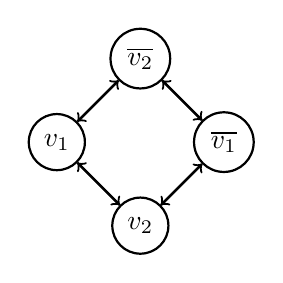
\begin{tikzpicture}[node distance={15mm}, thick, main/.style = {draw, circle}] 
\node[main] (1) {$v_1$}; 
\node[main] (2) [above right of=1] {$\overline{v_2}$}; 
\node[main] (3) [below right of=1] {$v_2$}; 
\node[main] (4) [above right of=3] {$\overline{v_1}$}; 
\draw[->] (4) -- (3); 
\draw[->] (2) -- (1); 
\draw[->] (1) -- (2); 
\draw[->] (3) -- (4); 
\draw[->] (1) -- (3); 
\draw[->] (2) -- (4); 
\draw[->] (4) -- (2); 
\draw[->] (3) -- (1); 
\end{tikzpicture}
\end{center}
\item Show: If there exists a directed path from $v$ to $u$ in  $\widetilde{G}$ for $u,v\in V$, then there also exists a path from $\overline{u}$ to $\overline{v}$.
	
	Let the path from $v$ to $u$ be $v\Rightarrow p_1 \Rightarrow p_2 \Rightarrow \dots \Rightarrow p_n \Rightarrow u$. By construction of  $\widetilde{G}$, if there is a $l_1\Rightarrow l_2$, then there is also $\overline{l_2}\Rightarrow \overline{l_1}$. Therefore, there is a path: $\overline{v}\Leftarrow \overline{p_1} \Leftarrow \overline{p_2} \Leftarrow \dots \Leftarrow \overline{p_n} \Leftarrow \overline{u}$. Hence, there also exists a path from $\overline{u}$ to $\overline{v}$.
\item Show: 2-SAT is \underline{not}-satisfiable if and only if there is a node $v\in V$ for which there exists both a directed path from $v$ to $\overline{v}$ as well as a directed path from $\overline{v}$ to $v$.

	Let the path from $v$ to  $\overline{v}$ be $v\Rightarrow p_1 \Rightarrow p_2 \Rightarrow \dots \Rightarrow l_1 \Rightarrow l_2 \Rightarrow \dots \Rightarrow p_n \Rightarrow \overline{v}$. If there is $l_1 \Rightarrow l_2$, then there is a claus $(\overline{l_1} \lor l_2)$. Consider the posiible values of $v$:
	\begin{itemize}
		\item $v$ = TRUE

		The edge from $l_i$ to $l_k$ represents that if $l_i$ is TRUE, then $l_k$ must be also TRUE. Let us divide our path into 2 paths: from $v$ to $l_1$ and from $l_2$ to $\overline{v}$. Hence, all literals in first path must be TRUE and in the second one must be FALSE. Since, $(\overline{l_1} \lor l_2)$ is a claus if it becomes FALSE $\mathcal{F}$ becomes not-satisfiable.
		\item $v$ = FALSE
		
		Exactly the same proof that $\mathcal{F}$ becomes not-satisfiable, but for a path from $\overline{v}$ to $v$.
	\end{itemize}
	\item Show by i)-iii): 2-SAT $\in \mathcal{P}$

	In order to show that 2-SAT$\in \mathcal{P}$ we need to show that we can check for the existance of a path from $\overline{v}$ to $v$ and from $v$ to $\overline{v}$ in a polynomial time. The search for this path is $O(N^2)$, since for every variable (N) are considered (N) clauses, which means the algorithm is polynomial. 
	\end{enumerate}
\end{enumerate}

\end{document}